% This file is the Latex source of the Big Data course project
% report. The project contributors are Ali Alavi, Rolf jagerman
% and Ken Tsay.
% The report is written by Ali Alavi, Rolf Jagerman, Ken Tsay.

%
\documentclass{llncs}
%

\usepackage{graphicx} % for importing images
\usepackage{caption}
\usepackage{subcaption} % for subfigures
\usepackage{amsmath}
\captionsetup{compatibility=false} % to make subfigures compatible with template

\usepackage{url} % for URL references
\urlstyle{same}
\usepackage{float} % helps with locating the 
\usepackage[T1]{fontenc}  % providing font encoding
% used for drawing the diagrams
%
\begin{document}
%
\mainmatter              % start of the contributions
\pretolerance=10000  % This avoids long lines
\pagestyle{headings}
%\hyphenation{}

%
\title{Automatic News Generation Based on Twitter}
%
\titlerunning{Automatic News Generation Based on Twitter}  % abbreviated title (for running head)
%                                     also used for the TOC unless
%                                     \toctitle is used
%
\author{Ali Alavi\inst{1} \and Rolf Jagerman\inst{1} \and
Tsay Kai-En\inst{1}}
%
\authorrunning{Ali Alavi, Rolf Jagerman and Tsay Kai-En} % abbreviated author list (for running head)
%
%
\institute{ETH Z\"urich, Z\"urich, Switzerland\\
\email{alavis@ethz.ch, \{rolfj, tsayk\}@student.ethz.ch}
}

\maketitle              % typeset the title of the contribution
%

\begin{abstract}
In this report, we describe our approach towards generating news topics based on twitter data. We tackle this problem by running a stochastic gradient descent classifier on a large set of news articles collected from different news agencies, and then using this classifier to classify twitter posts into three news categories: sports, politics, and technology. Then we tokenize these classified tweets in order to extract names and nouns used in each tweet. Finally we perform a time series analysis on these set of words and recognize top ten trending topics as news-worthy. We present the results in a web based interface. The results, especially in politics and sports category, bear resemblance with the trending topics as reported by news agencies.
\end{abstract}

\section{Introduction}

The authors were motivated by a simple question: can we generate more accurate and less biased news using twitter data in comparison to traditional news agencies? Would such a system have a potential of becoming an alternative to mainstream news sources? If so, such a system could be a more reliable source of unbiased news, which in turn will have immense effect on public awareness, knowledge and discourse.

Although there are many tools and websites, such as Google News, which automatically aggregate and present news articles, their data sources are  mainstream news agencies. We, on the other hand, want to use public posts as our data source, hence using collective knowledge of citizens as our news agency. Hence, the citizens will we be the audience as well as content providers.

In this model, every twitter user can play a small, yet collectively significant role in news gathering, and hence in generating valuable news articles, even without his or her knowledge. This is the main difference between our vision and that of citizen journalism, where citizens intend to produce a news headline, article or story. A concept we would like to call \textit{crowd-reporting}.

There is not much traditional techniques that can be used for realizing such system, since the core concept of this system makes use of big data collected from Twitter, something that no traditional technique can replace. Although we can think of using one or more data sources other than Twitter to achieve similar results.

\section{Contribution}
Current approaches to generate news based on Twitter focus on personal data for the most part. A system called "the tweeted times" is the closest thing we could find to our idea. It generates a news-paper type overview of your personal twitter account. This personalized approach however does not attempt to extract interesting news topics from the large twitter data stream. In our approach we first classify all available tweets and then perform time-series analysis on the results. A few works \cite{Go_Bhayani_Huang_2009,twitter-classifier} applied different machine learning methods (Naive Bayes Classifier, Support Vector Machine, etc) to classify tweets, but their data size was relatively small compared to us. Other works such as Trendsmap \cite{Trendmap}, shows you the latest trends from Twitter for anyplace in the world. However, they are doing data analysis on Twitter hashtags instead of the content of tweets. In our approach we are classifying the full contents of tweets into three categories and then automatically generating key terms of news based on these labeled tweets. This is a novel approach of which we could not find any previous research.

\section{Data model}
The twitter streaming API provides data in JSON format. It outputs a tweet as a JSON object on a single line. We copied this data storage format to our permanent data storage. That is: we have a JSON object representing a tweet on each separate line in our data files.

The Spark Map-Reduce framework naturally works with text data where each line represents a new element. By using functionality such as Spark's \texttt{textFile}, we can map each line of text, which represents a tweet, to a specific function. This makes using the data in a Map-Reduce context extremely easy.

\subsection{Data storage}
We stored around 600GB of the twitter stream data on Amazon S3. We used the s3cmd tool, which is a command line tool and client for uploading, retrieving and managing data in Amazon S3 \cite{s3cmd}. By integrating our data collection script with this tool, we can directly upload the twitter streaming data into the S3 bucket. This benefits the whole system because we can load the large data set using the S3 protocol into our Spark instances.

\subsection{Data processing platform}
The data processing platform we use is Apache Spark running on top of Amazon Elastic MapReduce (EMR). Initially we ran Spark on Amazon EC2 directly without using EMR. It turned out that the default configuration did not work well, and the executed tasks had a failure rate of about 50\%. For this reason, we decided to try the EMR platform. This platform has Spark pre-configured, which resulted in a 0\% failure rate for our tasks.

\section{System architecture}
The system architecture is depicted in Figure \ref{fig:architecture}. The main idea here is to train a classifier for several news topics using the news twitter accounts as training data. Then we use this classifier to predict the massive stream of public tweets into these news topics. Any tweets that are not classified as 'sports', 'politics' or 'technology' are discarded. This filters out most of the non-relevant tweets. Finally the predicted tweets are used to compute term frequencies over time and detect interesting news trends.

\begin{figure}
	\centering
	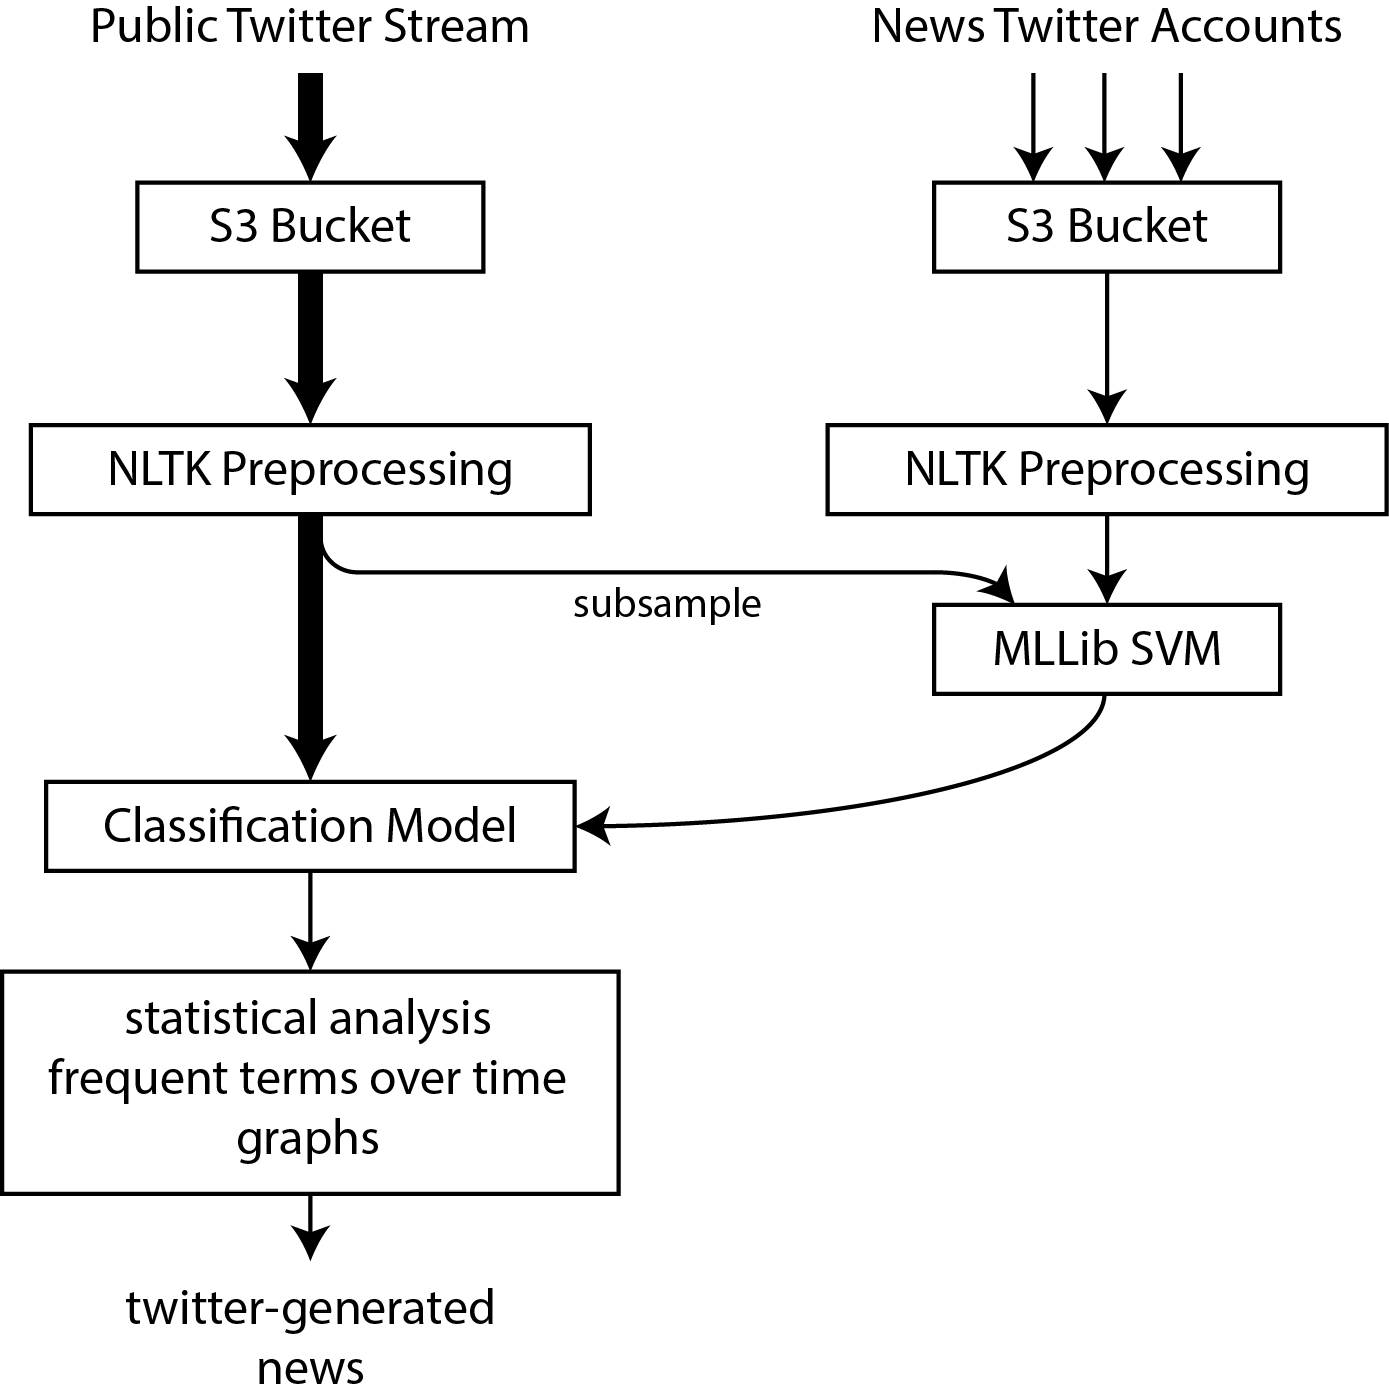
\includegraphics[width=0.72\textwidth]{images/system_arch.png} 
	\caption{The architecture of the system}
	\label{fig:architecture}
\end{figure}

The system is entirely build using python and we use the NLTK \cite{nltk} and Scikit-Learn \cite{scikit-learn} libraries to do the preprocessing. For each tweet we extract the text, tokenize it, stem it and turn it into a sparse feature vector by using the hashing trick. The classifier is trained using Spark's MLLib \cite{mllib}. Although we do not have sufficient training data to necessitate the use of MLLib's distributed learning, we use it to compute the predictions on our large twitter data set, which requires scalability.

After classifying the tweets and discarding most of the non-relevant ones we are left with a smaller data set. A single computer is sufficiently capable of performing the time-series analysis on this data set in less than an hour. The final results of this analysis are then used by a simple web interface to display the twitter generated news to the end user.

\section{Performance Measurements and Results}
The system is capable of classifying tweets and performing time-series analysis on them. In the first stage, the system classifies tweets as belonging to one of three possible categories: "sports", "politics" and "technology". These categories were chosen because they often contain news relevant information and have very little overlap in terms of terminology. It is important that this is scalable and highly performant because we are classifying our entire twitter data set (about $600\text{GB}$). In the second stage, a time-series analysis is performed on the resulting classified tweets. At this point, the total amount of data has been reduced significantly because most of the non-relevant tweets have been removed. The time-series analysis therefor runs on a single computer and takes less than one hour to complete.

\subsection{Execution time}
The Spark MapReduce platform reduces our tweet classification task into 10,702 smaller tasks. Each tasks gets approximately $\frac{600\text{GB}}{10702} = 57.4\text{MB}$ worth of data. Such a task takes on average $65.4$ ($\pm 20.6$) seconds to complete, which means a single machine can process about $0.87\text{MB}$ of data per second. This includes parsing twitter JSON, removing stop words and URLs, stemming text, feature hashing and classification. On 20 machines it is possible to compute $17.54\text{MB}$ per second. In total this adds up to an execution time of 10 hours on the entire data set. Adding more machines would further decrease this.

\subsection{Memory consumption}
Our classifier uses feature hashing and stochastic gradient descent. Feature hashing ensures that each tweet gets hashed into approximately 1 million features. Because every tweet is processed individually by the stochastic gradient descent algorithm and our feature space is of a fixed size we achieve a space complexity of $O(1)$.

\subsection{Solution quality}
To measure the quality of our news classifier we do not train on a part of our dataset, and instead only test on that part. Furthermore we randomly select tweets from the public twitter stream which we assume are not news-worthy or relevant. These tweets should not be classified in any of the categories. We are interested in optimizing the precision, recall and $F_1$-score. When the classifier scores high on these measures, we are confident in its ability to categorize new tweets.

\begin{table}[H]
	\begin{center}
		\begin{tabular}{|r|r|r|r|r|} \hline
			class  & precision   & recall & f1-score  & support \\ \hline
			technology    &   0.78 &     0.92  &    0.84   &  25343 \\
			sports   &    0.75   &   0.73   &   0.74   &   25343 \\
			politics   &    0.83  &    0.75   &   0.79   &   25343 \\
			avg / total  &     0.79   &   0.80  &    0.79   &  76029 \\ \hline
		\end{tabular}
	\end{center}
	\caption{Tweet classification performance over the three trained categories}
	\label{tbl:newclassifier}
\end{table}

The achieved $F_1$ score is on average 0.79. This is sufficient for the purpose of removing non relevant tweets. The time-series analysis performed on the resulting tweets is capable of handling a small amount of noise that the classifier might output.

\section{Conclusion}
The research question of this project is whether or not it is possible to predict the news using public tweets. In particular we are interested in the quality of the predicted news as it relates to existing news sources. We simplify this problem by focusing on three specific topics of news: "politics", "sports" and "technology".

The system we have constructed has provided us with several interesting insights. Political news gave us some of the best results. Obama's announcement about the new immigration law for example was very clearly reflected in the results. Sports news seems particularly tailored to predicting when a match is ongoing and its score. News in the technology category gave the worst results, as it is for example very difficult to predict whether a tweet containing the word "iPhone" is actually relevant (such as the release of the new iPhone) or not interesting at all (people complaining about their iPhones).

During the construction of the system we encountered several difficulties. After installing spark on amazon EC2, we noticed that when running a simple map-reduce word count program on a large data set about 50\% of all tasks were failing and had to be restarted. As we were unsure what the cause of this problem was, we decided to do a clean install of Spark using Amazon's EMR. Because this Spark installation was specifically tailored for EMR, it worked much better and we had a 0\% failure rate on the tasks. Another difficulty was collecting enough training data. Getting twitter data is easy, but getting news-relevant twitter data is rather difficult. We settled for using the news agencies' twitter accounts as a source of training data. Overall we think more training data would have improved the solution quality. It was however difficult to obtain more training data as we exhausted all of the known large news agencies.

In retrospect we should have tried different and perhaps more specific categories for the classification of the news. In particular, the technology category made it very difficult to find any news-worthy topics.

Given more time it would be interesting to try additional features, such as the geolocation of tweets, the number of retweets, followers or other interesting measures. Also, the collection of more training data from sources other than twitter could have improved the solution quality and is a worthwhile pursuit.

\bibliographystyle{plain}
\bibliography{report.bib}

\end{document}